\chapter{Implementácia}

\section{Vývoj s pomocou príkazového riadku}

\section{Smerovanie}

\section{Modely}

\section{Controllery}

\section{Views}
\subsection{HTML a ERB}
\subsection{CSS}
\subsection{JavaScript}

\section{Spracovanie úloh na pozadí}

\section{Generovanie PDF prehľadov}
\section{Odosielanie e-mailov}

\clearpage
\section{Užívateľské rozhranie}

\subsection{Prihlásenie a registrácia}

Pred začatím používania aplikácie sa musí užívateľ najprv prihlásiť alebo registrovať. Všetky podstránky aplikácie sú zabezpečené a užívateľ je presmerovaný pokiaľ nie je prihlásený.

\begin{figure}[!htb]
  \centering
    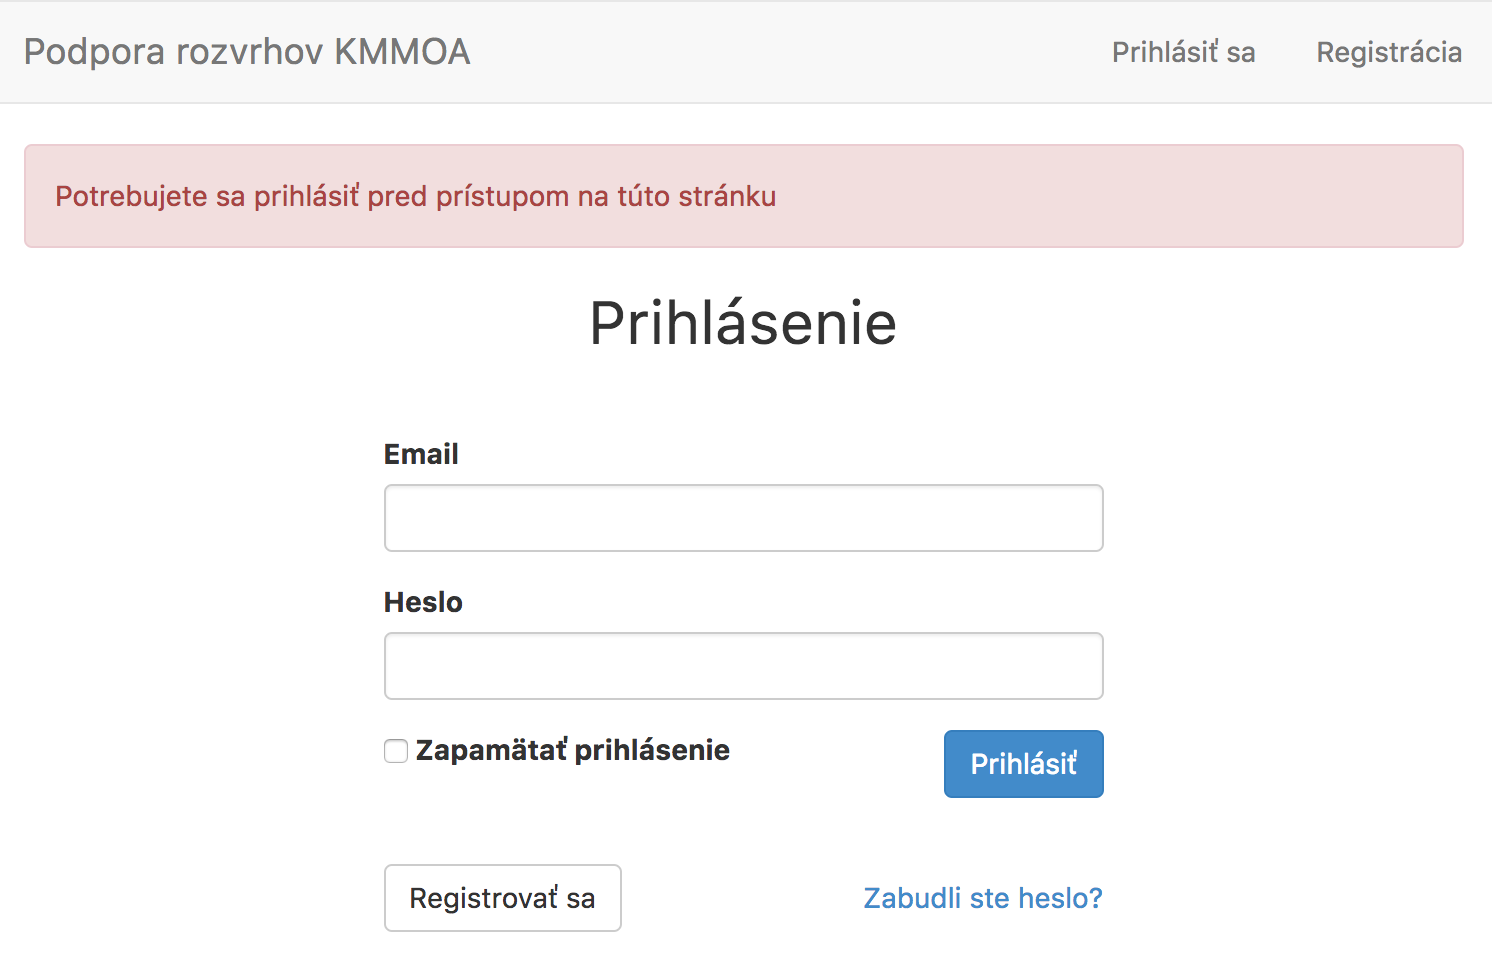
\includegraphics[width=1\textwidth]{content/images/login}
    \caption{Rozhranie pre prihlásenie do aplikácie.}
\end{figure}

Užívatelia si taktiež môžu prenastaviť heslo pomocou emailu ak ho náhodou zabudli. Na zadaný email sa zašle link na stránku, kde užívateľ môže heslo zmeniť. Registrácia sa navyše dá kedykoľvek vypnúť administrátorom použitím premennej prostredia.

\clearpage
\section{Turbolinks}

Turbolinks je JavaScript knižnica, ktorá robí navigáciu po webovej stránke rýchlejšou. Poskytuje rýchlostné benefity single-page aplikácie, bez pridanej komplexnosti iných JavaScript frameworkov. Vykreslenie celej HTML stránky môže bez obáv prebiehať na strane servera. Keď chce užívateľ prejisť na inú stránku pomocou kliknutia na link Turbolinks pomocou AJAX-u vyzdvihne danú stránku a vymení obsah tagu \emph{<body>} a zlúči obsah v tagoch \emph{<head>}, to všetko bez potreby znovu načítať celú stránku. \citep{web:turbolinks}

\section{Problémy pri implementácii a ich riešenie}
\subsection{N+1 queries}

Pri načítaní niektorých prehľadov, ako napríklad prehľad vyučujúcich sa začali v logoch servera objavovať dlhé zoznamy SQL dotazov. Ako prvé som si všimol, že je to spôsobené iteráciou cez vzťahy kolekcie modelov. Ako napríklad:

\begin{minted}{ruby}
@techers = Teacher.all()

@teachers.courses.each do |course|
  puts course.title
end
\end{minted}

To spôsobí, že pre každý model vo vzťahu je načítaný samostatným SQL selectom, čo ale nechceme, pretože to spôsobuje nadmerné zaťaženie databázy. Po zamyslení nad týmto problémom je jasné, že musíme načítať modely aj všetky ich vzťahy cez ktoré chceme iterovať naraz s použitím JOIN-u.
Našťastie ale vývojári ActiveRecord-u na toto správanie mysleli a nezabudli ho implementovať. Riešenie je veľmi jednoduché:

\begin{minted}{ruby}
@techers = Teacher.includes(:courses).all()

@teachers.courses.each do |course|
  puts course.title
end
\end{minted}

Pri načítaní modelov použijeme funkciu \emph{includes()} do ktorej môžeme napísať symboly, ktoré reprezentujú jednotlivé vzťahy. Po skontrolovaní logov teraz vidíme, že pri načítaní náhľadu sa teraz spustí iba 1 SQL query.

\subsection{Dlhé časy požiadaviek}

Toto správanie je spôsobené tým, že funkcia v controlleri trvá dlhšie ako je obvyklé a tým zdržiava navrátatenie odpovede užívateľovi.
Problém sa vyskytol najmä pri odosielaní e-mailov a generovaní PDF prehľadov. Ide o jednoduchý problém, ktorý sa dá vyriešiť niekoľkými spôsobmi. 

V aplikácii je tento problém vyriešený použitím balíčka (\emph{\texttt{gem 'delayed\_job'}}), ktorý vykonáva dlho-trvajúce funkcie na pozadí. Balíček má v databáze svoju tabuľku, do ktorej ukladá všetky funkcie, ktoré má vykonať. 

Avšak, tento balíček sa musí spustiť externe cez príkazový riadok, preto je múdre pridať aj balíček (\emph{\texttt{gem 'daemons'}}) aby sme mohli tento proces daemonizovať. Spustíme ho zo zložky aplikácie príkazom:

\begin{minted}{bash}
$ bin/delayed_job start
\end{minted}

Neskôr treba na produkčnom serveri tento skript nalinkovať aby sa automaticky spúšťal pri štarte/reštarte servera.